\documentclass[times, utf8, seminar]{fer}
\usepackage{booktabs}
\usepackage{graphicx}
\usepackage{csquotes}
\usepackage{listings}
\usepackage{courier}
\graphicspath{{slike/}}

\lstset{basicstyle=\footnotesize\ttfamily,breaklines=true}
\lstset{numbers=left,frame=single}

\begin{document}

\title{Preporučiteljski sustav Pixie}

\author{Petar Šegina}

\voditelj{Raspodijeljena obrada velike količine podataka}

\maketitle

\tableofcontents

\chapter{Uvod}

Preporučiteljski sustav je sustav čija je zadaća predvidjeti korisnikov odabir nekog izbora\footnote{\cite{mmd}}. Takvi sustavi čine veoma važnu značajku modernih mrežnih usluga, nudeći korisnicima zanimljiv, bitan i njima personaliziran sadržaj. Takav sustav također može povećati interakciju korisnika sa sadržajem za kojeg potencijalno nije ni svjestan da postoji, a koji bi mu mogao biti od interesa. Tako jedan glazbeni web dućan može povećati prodaju preporučivanjem pjesama i albuma sličnima onima za koje je korisnik pokazao interes, dok jedan portal s vijestima može korisniku preporučiti slične i zanimljive vijesti kako bi ga duže zadržao na samom portalu i povećao prihod od prikaza reklama.

Pinterest\footnote{\url{https://pinterest.com}} je moderna web usluga koja svojim korisnicima omogućuje otkrivanje novih i relevantnih ideja za izradu kreativnih projekata -- od kuharskih recepata pa do dizajna interijera. Riječima njihovog inženjerskog tima:

\begin{displayquote}
		  \textit{At Pinterest, a primary engineering challenge is helping people discover and do things every day, which means serving the right idea to the right person at the right time.}\footnote{\cite{medium-article}}
\end{displayquote}

Pinterest je u svojoj srži preporučiteljski sustav te je važno da kao takav može dati korisne preporuke u dovoljno kratkom vremenu kako bi svojim korisnicima ponudio što veću vrijednost. Zbog veličine podataka i vremenskih zahtjeva kojima Pinterest barata, a koje ćemo iznijeti u nastavku, postojeća rješenja pokazuju značajne nedostatke te je Pinterest za svoje potrebe odlučio napraviti vlastiti preporučiteljski sustav, naziva Pixie, koji se pokazao izrazito učinkovitim. Nad njihovim skupom podataka -- bipartitnim grafom od 3 milijarde čvorova povezanih sa 17 milijardi bridova, jedan Pixie poslužitelj može poslužiti 1.200 zahtjeva po sekundi sa latencijom u 99-om centilu unutar 60 milisekundi. S poslovne strane se Pixie također pokazao kao uspjeh jer je povećao i relevantnost preporuka koje se korisnicima nude i time povećao angažman korisnika za do 50\%\footnote{\cite{DBLP:journals/corr/abs-1711-07601}}.

U nastavku dajemo pregled preporučiteljskog sustava Pixie -- problema kojeg on pokušava riješiti, nekolicinu inovativnih pristupa rješavanju tog problema, primjer ostvarenja tih pristupa u programskom jeziku Kotlin\footnote{\url{https://kotlinlang.org}} te rezultate koje to ostvarenje daje.

\chapter{Problem}

\section{Generalizirani model}
Opišimo prvo općeniti problem preporučivanja koji pokušavamo riješiti. Model kojeg iznosimo ovdje inspiriran je formalnim modelom iznesenim u \cite{avsp-recommender}.

Krenimo od sustava koji se sastoji od dva skupa -- skupa korisnika \textit{K} i skupa predmeta \textit{P} s kojima korisnik može međudjelovati. Dodatno, svaki korisnik može za neki predmet iskazati koliko mu je taj predmet zanimljiv, što možemo modelirati funkcijom zanimljivosti $z = K \times P \to \mathbb{R}$ koja za danog korisnika i dani predmet vraća koliko je tom korisniku taj predmet zanimljiv.

Ukoliko za danog korisnika sortiramo skup predmeta po funkciji zanimljivosti, dobivamo listu predmeta poredanih po zanimljivosti za tog korisnika $P_k = sorted(P, z_k)$. Temeljem ove liste korisniku možemo preporučiti novi sadržaj uzimajući, primjerice, prvih 5 elemenata te liste.

Ovakav jednostavan model pokazuje temeljni zahtjev od preporučiteljskog sustava -- da na temelju poznatih informacija o korisniku može za njega preporučiti relevantan sadržaj. 

No, postoje određeni izazovi kojih je važno biti svjestan. Prvo je nepoznavanje funkcije z -- korisnik će eksplicitno izraziti zanimljivost tek za veoma maleni podskup predmeta. Kako bi mogli ponuditi preporuke, morati ćemo zanimljivost za ostale predmete procijeniti. Drugi bitan izazov je veličina skupa podataka -- $K \times P$ može biti velikih dimenzija, reda veličine $10^6 \times 10^6$ pa nećemo moći naivno obraditi cijeli skup podataka, već će biti nužno usredotočiti se na tek maleni podskup istih.

Postoje razni pristupi rješavanju ovog problema, od čega su možda najpopularniji preporučivanje temeljeno na sadržaju te suradničko filtriranje, koji su također dostupni kao gotovi algoritmi u programskom okviru \textit{Apache Mahout}\footnote{\cite{rovkp-mahout}}.

\section{Pinterestov problem}

Pogledajmo sada problem preporučivanja kojeg Pinterest pokušava riješiti. Vidjet ćemo da se određena svojstva specifična njihovom problemu mogu iskoristiti za bolje i efikasnije generiranje preporuka.

\subsection{Problem preporučivanja}

U Pinterestovom skupu podataka postoje dva tipa entiteta - pin (\textit{pribadača, značka}) i board (\textit{ploča}). Svaki pin može biti povezan s više boardova i svaki board može imati više pinova, tj.\ relacija među njima je oblika N-N.

Te podatke možemo prikazati grafom na način da čvorove predstavljaju pinovi i boardovi, a bridove veze među njima. Kako ne postoji veza pin-pin niti veza board-board, navedeni graf je bipartitan. Kako su veze također dvosmjerne, graf je i neusmjeren.

\begin{figure}[h]
	\centering
	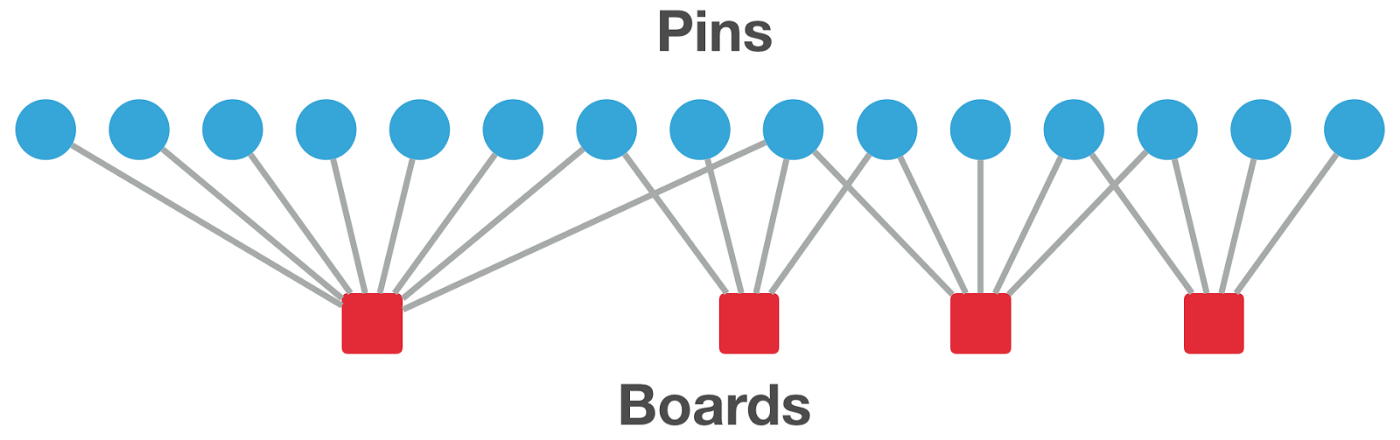
\includegraphics[width=\textwidth]{pins_boards_graph}
	\caption{Graf podataka}
	\cite{medium-article}
	\label{fig:pins_boards}
\end{figure}

Kada korisnik posjeti pin ili board, želja nam je pokušati preporučiti relevantne pinove kako bi korisnik mogao nastaviti svoju potragu u svome smjeru. Tako od preporučiteljskog sustava želimo da nam za dani pin i dani graf nađe druge pinove koji će korisniku biti zanimljivi.

Dodatno, ne želimo preporuku stvoriti samo na temelju jednog pina, već više njih koje je korisnik posjetio, s time da veći naglasak želimo staviti na one pinove koje je korisnik posjetio nedavno. Konačno, kako bi još više poboljšali preporuke, veći naglasak želimo staviti na one pinove koji bi korisniku mogli biti zanimljivi po nekim drugim parametrima koji nisu očiti iz grafa -- kao što su jezik sadržaja ili tema oko koje je sadržaj grupiran.

\subsection{Razmjer podataka i vremenski zahtjevi}

Važno je također posebnu pažnju skrenuti i na razmjer podataka kojima Pinterest barata. U svome radu\footnote{\cite{DBLP:journals/corr/abs-1711-07601}} ističu kako njihov graf sadrži 7 milijardi čvorova i 100 milijardi bridova. U radu također ističu i broj korisnika koji nadmašuje 200 milijuna.

Također treba istaknuti i vremenske zahtjeve na preporučiteljski sustav -- Pinterestu je važno da se preporuke mogu generirati u stvarnom vremenu, kako korisnik koristi sustav. Zbog toga je važno da izračun preporuka bude brz te je već čekanje od jedne sekunde previše i znatno bi narušilo krajnje korisničko iskustvo.

S ovim svime na umu, vidimo jasnu motivaciju zašto napraviti vlastiti preporučiteljski sustav -- oblik i količina podataka te vremenski zahtjevi nisu prikladni za pristup poput suradničkog filtriranja čije je vrijeme osvježavanja znatno duže i čiji prostorni zahtjevi nisu prikladni za red veličine miljardi.

\chapter{Rješenje}

Kako bi riješili navedeni problem, u Pinterestu su primijenili nekoliko inovativnih tehnika koje iskorištavaju oblik podataka kako bi generirale brz i relevantan odgovor.

\section{Jednostavna nasumična šetnja}

Algoritam Pixie zasnovan je na jednostavnoj nasumičnoj šetnji po grafu $G = (P, B, E) $.

Za dani graf G i početni pin $p \in P$, algoritam vrši nasumičnu šetnju u slijedećim koracima:

\begin{enumerate}
	\item Generiraj brojač $V: P \to \mathbb{N}$ s pretpostavljenom vrijednošću 0
	\item Za dani p nasumično odaberi $e_1 \in E$ koji povezuje p s nekim $b \in B$
	\item Za b nasumično odaberi $e_2 \in E$ koji povezuje b s nekim $p_2 \in P$
	\item Inkrementiraj $V[p_2]$
	\item Nastavi od koraka 2.\ koristeći $p_2$ kao početni pin
\end{enumerate}

Jasno je da ovaj algoritam neće nikad završiti pa zato ograničavamo duljinu šetnje na odabrani broj koraka N. Nakon što algoritam završi, u brojaču V imamo broj posjećenosti svakog pina. Kako je vjerojatnije da će nasumična šetnja češće proći pinovima koji su početnom pinu bliski, broj pogodaka možemo koristiti kao mjeru sličnosti i kao preporuku vratiti one pinove koji su najčešće posjećeni.

Prednosti ovog algoritma su jednostavnost i performanse -- vrijeme izvođenja je konstantno u odnosu na veličinu grafa te ovisi samo o duljini šetnje, N.

No, za uspješan rad algoritma, potrebno je na ovu nasumičnu šetnju dodati još poneka poboljšanja.

\section{Dodavanje pristranosti nasumičnoj šetnji}

Primijetimo da prethodni algoritam ne uzima u obzir nikakva saznanja o korisniku. Za dva korisnika, $u_1$ i $u_2$, i isti početni pin $p$, preporuka će, ignoriravši nasumičnost šetnje, biti ista. Kako nam je želja dobiti preporuke koje će biti personalizirane za korisnika, potrebno je šetnju \textit{pogurnuti} u pravom smjeru. Prilika za to napraviti je prilikom odabira brida kojim će šetač proći. Umjesto nasumičnog odabira gdje svaki brid ima jednaku vjerojatnost da bude izabran, vjerojatnosti odabira se mogu izraziti kao pripadne težine bridova koje ovise o svojstvima trenutnog korisnika i predmeta koji se razmatra.

\section{Upiti sa više pinova}
\label{multipin}

Kako bi se korisnika još bolje modeliralo, uz trenutni pin kojeg korisnik pregledava možemo uzeti u obzir i povijest pinova koje je korisnik pregledavao. Tako umjesto jednog upita q izvršimo skup upita Q i za svakog izračunamo pripadni brojač $V_q$.

Na kraju je potrebno dobivene brojače kombinirati. Brojače bi mogli kombinirati običnom sumom ili prosjekom, no nije svaki upit jednak. Naime, ako je početni pin jako povezan (ako se radi o čvoru visokog stupnja), biti će potrebno napraviti više koraka kako bi značajnost brojača bila jednaka onom dobivenom kretanjem od čvora niskog stupnja. U suprotnom bi preporuke generirane čvorovima niskog stupnja dominirale nad preporukama čvorova visokih stupanja, iako su potonji zbog svoje veće povezanosti u grafu značajniji.

Kako bi se riješio ovaj problem, za svaki upit q računa se faktor razmjera (\textit{scaling factor}) na slijedeći način:

\begin{centering}
		  $ k = |E(q)| $ \\
		  $ C = max_{p \in P}|E(p)| $ \\
		  $ s_q = k * (C - log(k)) $ \\
        k -- stupanj pin čvora upita \\
		  C -- najveći stupanj nekog pin čvora 
		  \par
\end{centering}

Na temelju tog faktora, računa se duljina šetnje pojedinog pina, $N_q$ temeljem ove formule:

\begin{centering}
	$ N_q = w_qN\frac{s_q}{\sum_{r \in Q}s_r} $\par
\end{centering}

Distribucija duljine šetnji je sada takva da će šetnje koje počinju u čvorovima visokog stupnja imati razmjerno veću duljinu u odnosu na šetnje koje počinju u čvorovima niskog stupnja, ali će i dalje i ti čvorovi imati dovoljno duge šetnje.

Za potrebe ilustracije, generirali smo nasumičan skup od 40 čvorova stupnja između 1 i 100 i za svakog izračunali $N_q$ uz $N = 1000$ i $w_q = 1$. Vidljivo je da broj koraka raste linearno sa stupnjem čvora. Čvorovima stupnja 2 dodijeljena je šetnja duljine jednog koraka, a čvorovima stupnja 96 šetnja duljine 53. Korišteni skup podataka dostupan je u popratnoj datoteci \textit{degree\_length\_chart.ods}.

\begin{figure}[h]
	\centering
	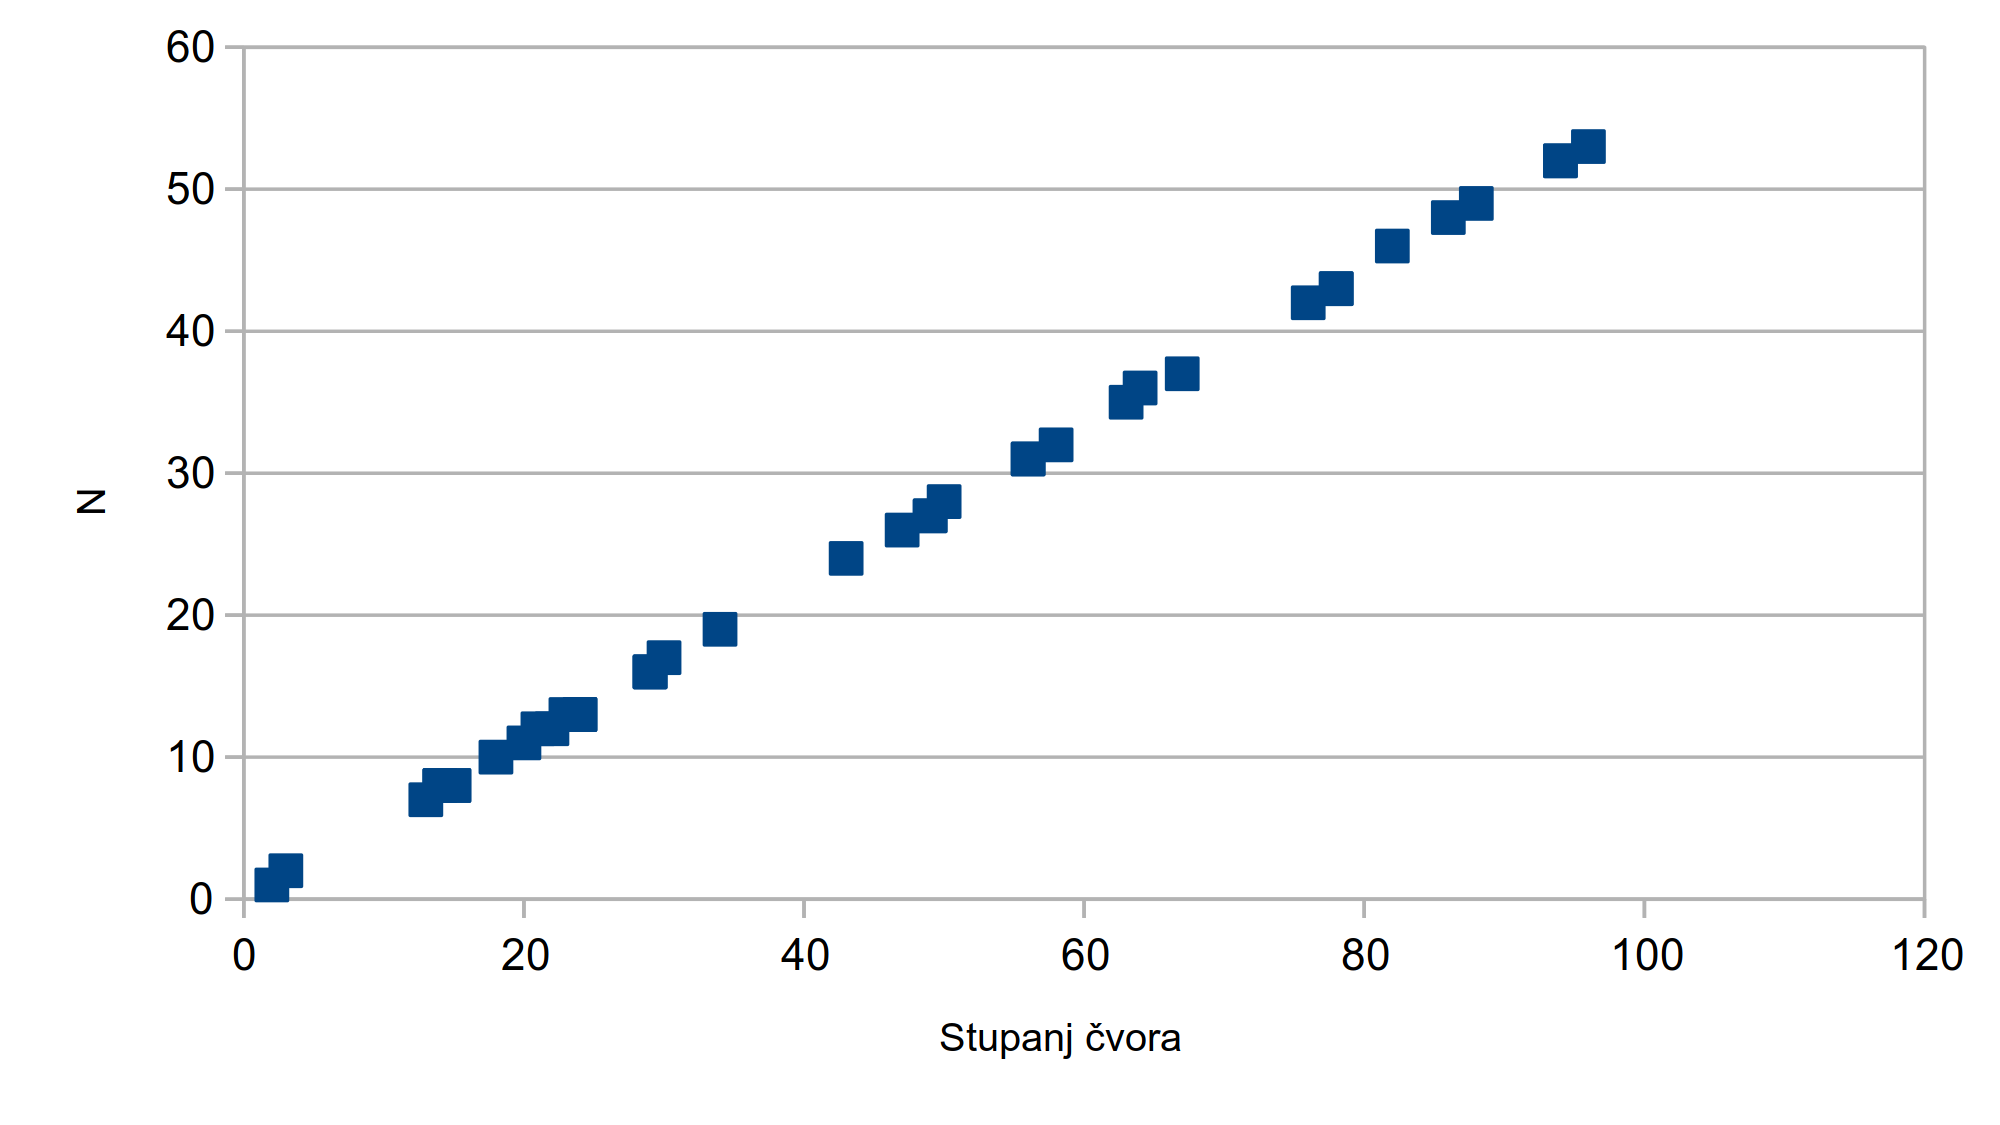
\includegraphics[width=\textwidth]{degree_chart}
	\caption{Odnos $k_q$ i $N_q$ za nasumično generiran skup podataka}
	\label{fig:pins_boards}
\end{figure}

\section{Poticanje pinova koji se pojavljuju više puta}
\label{boosting}

Nakon što smo odredili duljine šetnji, preostaje pitanje kako na kraju kombinirati dobivene $V_q$ u jedan konačni brojač na temelju kojeg ćemo generirati preporuke. Intuicija je da su oni pinovi koji su povezani sa više pinova u Q također i relevantniji krajnjem korisniku, tj.\ oni pinovi koje je više različitih šetnji posjetilo su značajniji za konačni rezultat. Jednostavnim zbrajanjem $V_q$ bi izgubili ovu informaciju pa umjesto toga ukupan broj \textit{pogodaka} za pin p računamo ovako:

\begin{centering}
		  $$ V[p] = (\sum_{q \in Q}{\sqrt{V_q[p]}})^2 $$
		  \par
\end{centering}

Na ovaj način će pinovi koji se pojavljuju u više šetnji biti \textit{nagrađeniji}. Primjerice, ako se jedan pin pojavljuje u dvije šetnje po 100 puta, njegov rezultat će biti $ (\sqrt{100} + \sqrt{100})^2 = 400 $ što je znatno više od jednog pina koji se u jednoj šetnji pojavljuje 200 puta, čiji će rezultat tada biti $ \sqrt{200}^2 = 200 $.

\section{Rano zaustavljanje}
\label{early-stop}

Primijetimo da šetnje imaju konstantnu duljinu koja ovisi o početnom čvoru. No, možemo postići značajnu uštedu vremena ako odlučimo stati sa šetnjom ranije ako se to čini kao dobra ideja.

Naivan kriterij za zaustavljanje može biti konvergencija rješenja - top N kandidata se nije promijenilo u zadnjih k koraka. No, kako praćenje te informacije može biti skupo (pa čak i skuplje od same šetnje), Pixie uvodi jednostavnu heuristiku - šetnju zaustavljamo kada je bar $n_p$ pinova posjećeno bar $n_v$ puta. Brojevi $n_p$ i $n_v$ direktno utječu na kvalitetu rezultata i trajanje algoritma pa ih je potrebno pažljivo odabrati, a njihov odabir ovisi o skupu podataka koji se obrađuje. Primjera radi, Pinterest na svom skupu podataka za $n_p=2.000$ i $n_v=4$ postiže sličnost od 84\% sa rezultatom bez ranog zaustavljanja, a pritom smanjuje vrijeme izvršavanja upita na trećinu.

\section{Smanjivanje grafa}

Konačno, kao veoma bitan korak pokazalo se i smanjivanje samog grafa (\textit{graph pruning}) kao oblik predobrade podataka. Sam postupak uvelike ovisi o skupu podataka nad kojim se primijenjuje. U Pinterestovom slučaju svelo se na heuristiku uklanjanja čvorova sa visokom entropijom te, za pojedinačne pinove, uklanjanja onih bridova koji vode na boardove koji imaju najmanju sličnost sa danim pinom.

U Pinterestovom slučaju ovaj se postupak itekako isplatio -- sa 7 milijardi čvorova i 100 milijardi bridova, graf je smanjen na 3 milijarde čvorova (43\%) i 17 milijardi bridova (17\%). Dodatno, smanjenje grafa je također dovelo i do poboljšanja u kvaliteti preporuka u iznosu od 58\%, što je posljedica primijenjene heuristike koja sama po sebi uklanja manje relevantne bridove, koji onda neće ni biti posjećeni.

\chapter{Ostvarenje}

U nastavku opisujemo jednostavnu implementaciju osnovnih načela preporučiteljskog sustava Pixie u programskom jeziku Kotlin.

\section{Osnovne strukture podataka}

Definirajmo prvo osnovne strukture podataka koje ćemo koristiti. Pinove i boardove ćemo predstaviti jednim brojem kako bi ih kasnije mogli pratiti.

\begin{lstlisting}
data class Pin(val id: Int)
data class Board(val id: Int)
\end{lstlisting}

Također definirajmo i brojač koji će biti rezultat šetnji kao preslikavanje iz Pina u broj posjeta tog Pina.

\begin{lstlisting}
typealias Counter = Map<Pin, Int>
\end{lstlisting}

Kako će naš algoritam većinu vremena provesti šetajući između čvorova, definirajmo graf tako da on, uz pinove i boardove, sadrži i mapiranja koja opisuju povezivanja među njima. Iako nam uređaj nije bitan, mapiranja definiramo kao \textit{List} umjesto kao \textit{Set} jer nam je za šetnju potrebna mogućnost nasumičnog pristupa elementima.

\begin{lstlisting}
data class AdjacencyGraph(
        val pins: List<Pin>,
        val boards: List<Board>,
        val pinsToBoards: Map<Pin, List<Board>>,
        val boardsToPins: Map<Board, List<Pin>>
)
\end{lstlisting}

Definirajmo i pomoćne konstante koje će predstavljati parametre našeg generiranog skupa podataka te osnovnog broja koraka šetnje. Broj boardova, pinova i bridova biramo u jednakom omjeru kao što se nalazi u Pinterestovom reduciranom skupu podataka, ali biramo brojeve nekoliko redova veličina manje kako bi uštedjeli na vremenu potrebnom za generiranje i evaluiranje podataka.

\begin{lstlisting}
const val NUM_PINS = 2 * 10e4.toInt()
const val NUM_BOARDS = 1 * 10e4.toInt()
const val NUM_EDGES = 17 * 10e4.toInt()
const val NUM_STEPS = 100000
\end{lstlisting}

Definirajmo i pomoćnu \textit{Random} instancu sa definiranom \textit{seed} vrijednošću kako bi naši eksperimenti bili deterministični.

\begin{lstlisting}
val random = Random(9932L)
\end{lstlisting}

Nadalje, definirajmo nekoliko pomoćnih funkcija. Prvo, funkcija za nasumičan odabir elementa iz liste.

\begin{lstlisting}
private fun <T> List<T>.sample() = this[random.nextInt(size)]
\end{lstlisting}

Zatim definirajmo funkciju za dohvat top k elemenata iz brojača.

\begin{lstlisting}
private fun Counter.top(k: Int) = this
        .toList()
        .sortedByDescending { it.second }
        .take(k)
\end{lstlisting}

Te, nastavno, funkciju za ispis top k elemenata brojača.

\begin{lstlisting}
private fun Counter.printTop(k: Int) = top(k).forEach {
		  System.out.printf(" %s - %d%n",
		  	it.first, it.second)
}
\end{lstlisting}

Konačno, definirajmo pomoćnu funkciju koja će generirati skup podataka nad kojim ćemo izvršiti algoritam. Generirati ćemo potreban broj pinova i boardova i zatim ih na nasumičan način spojiti bridovima. Važno je napomenuti da bi u ovom postupku zbog vjerodostojnosti simulacije bilo korisno modelirati razdiobu histograma stupnja čvorova tako da ona odgovara stvarnim podacima, ali to u ovom primjeru preskačemo jer nemamo pristup toj informaciji o stvarnim podacima.

\begin{lstlisting}
fun generateData(): AdjacencyGraph {
    val pins = (1..NUM_PINS).map { Pin(it) }
    val boards = (1..NUM_BOARDS).map { Board(it) }

    val pinsToBoards = HashMap<Pin, MutableList<Board>>(NUM_EDGES)
    val boardsToPins = HashMap<Board, MutableList<Pin>>(NUM_EDGES)

    (1..NUM_EDGES).forEach {
        val pin = pins.sample()
        val board = boards.sample()

        pinsToBoards.computeIfAbsent(pin) { ArrayList() }
        boardsToPins.computeIfAbsent(board) { ArrayList() }

        pinsToBoards[pin]!!.add(board)
        boardsToPins[board]!!.add(pin)
    }

    return AdjacencyGraph(pins, boards, pinsToBoards, boardsToPins)
}
\end{lstlisting}

\section{Jednostavna nasumična šetnja}

Implementirajmo sad običnu nasumičnu šetnju nad danim grafom. Funkcija kao parametar prima skup podataka, početni pin te gornji broj koraka, a kao rezultat vraća popunjeni brojač.

\begin{lstlisting}
fun simpleRandomWalk(
	graph: AdjacencyGraph,
	startingPin: Pin,
	numberOfSteps: Int
): Counter {
    val counter = HashMap<Pin, Int>()

    var step = 0
    var pin = startingPin

    while (step < numberOfSteps) {
        val board = graph.pinsToBoards[pin].orEmpty().sample()
        val otherPin = graph.boardsToPins[board]!!.sample()

        val oldCount = counter.getOrDefault(otherPin, 0)
        counter[otherPin] = oldCount + 1
        pin = otherPin
        ++step
    }

    return counter
}
\end{lstlisting}

Sada možemo pokrenuti jednostavan eksperiment definiranjem funkcije \textit{main}.

\begin{lstlisting}
fun main(args: Array<String>) {
    val start = System.currentTimeMillis()
    System.out.printf("Generating dataset with %d pins, %d boards and %d edges%n", NUM_PINS, NUM_BOARDS, NUM_EDGES)
    val data = generateData()
    System.out.printf("Done in %d%n", System.currentTimeMillis() - start)

    val startingPin = data.pinsToBoards.keys.toList().sample()

    System.out.printf("Starting pin is %s%n", startingPin)

    val randomWalkTime = System.currentTimeMillis()
    System.out.printf("Starting simple random walk with %d steps%n", NUM_STEPS)
    val randomWalkResult = simpleRandomWalk(data, startingPin, NUM_STEPS)
    System.out.printf("Done in %d%n", System.currentTimeMillis() - randomWalkTime)
    randomWalkResult.printTop(10)
}
\end{lstlisting}

Izvršavanjem nasumične šetnje mijenjajući NUM\_STEPS dolazimo do slijedećih rezultata:

\begin{center}
		  \begin{tabular}{ |r|r| }
					 \hline
					 N & Vrijeme izvršavanja (ms) \\
					 \hline
					 1000 & 3 \\
					 \hline
					 10000 & 17 \\
					 \hline
					 100000 & 137 \\
					 \hline
		  \end{tabular}
\end{center}

Vidljivo je da vrijeme izvršavanja raste otprilike linearno, što je i očekivano. Također vidimo i da je gornja granica za broj koraka šetnje na našem računalu (Intel Core i5-2520M) reda veličine $10^5$. Sve više od toga bi trajalo predugo za preporuke u stvarnom vremenu. 

\section{Dodavanje pristranosti nasumičnoj šetnji}

U trenutnoj implementaciji prilikom svakog odabira svaki brid ima jednaku vjerojatnost biti odabran. Dodajmo sad mogućnost definiranja pristranosti šetnji kako bi povećali vjerojatnost odabira nekih zanimljivih bridova.

Prvo, definirajmo metodu koja će generirati težine bridova. Generirane težine će biti između 0 i 1, a kako su sve veze dvosmjerne, dovoljno je kreirati težine za bridove u jednom smjeru.

\begin{lstlisting}
fun generateWeights(pinToBoards: Map<Pin, List<Board>>) = pinToBoards.flatMap { (pin, boards) ->
    boards.map { board ->
        (pin to board) to random.nextDouble()
    }
}.toMap()
\end{lstlisting}

Iduće, potrebno je uzeti generirane težine u obzir prilikom odabira brida kojim će se krenuti. U implementaciji naše šetnje potrebno je samo promijeniti metodu \textit{sample} tako da ona umjesto uniformnog odabira radi \textit{roulette wheel selection}\footnote{\url{https://en.wikipedia.org/wiki/Fitness_proportionate_selection}} nad otežanim bridovima.

U tu svrhu, uvedimo novu, generaliziranu, funkciju \textit{sample} koja će vršiti ruletni odabir nad proizvoljnom listom podataka i odgovarajućom mapom težina.

\begin{lstlisting}
private fun <T, R, V, U> List<T>.sample(
        startingElement: R,
        weights: Map<Pair<V, U>, Double>,
        combiner: (R, T) -> Pair<V, U>
): T {
    val totalWeight = map { weights[combiner(startingElement, it)]!! }.sum()
    val selectedWeight = random.nextDouble() * totalWeight

    var traversedWeight = 0.0
    forEach {
        traversedWeight += weights[combiner(startingElement, it)]!!

        if (traversedWeight >= selectedWeight) {
            return it
        }
    }
    throw RuntimeException("Roulette wheel selection failed to select an element")
}
\end{lstlisting}

Sada je implementacija konkretnih funkcija \textit{sample} za odabir pinova i bridova jednostavna -- dovoljno je pozvati generaliziranu funkciju \textit{sample} s odgovarajućim podacima.

\begin{lstlisting}
private fun List<Board>.sample(startingPin: Pin, weights: Map<Pair<Pin, Board>, Double>): Board =
        sample(startingPin, weights) { i, j -> Pair(i, j) }

private fun List<Pin>.sample(startingBoard: Board, weights: Map<Pair<Pin, Board>, Double>): Pin =
        sample(startingBoard, weights) { i, j -> Pair(j, i) }
\end{lstlisting}

Konačno, za implementaciju šetnje s pristranosti, dovoljno je promijeniti \textit{sample} pozive. U nastavku dajemo cjelovitu implementaciju metode.

\begin{lstlisting}
fun weightedRandomWalk(graph: AdjacencyGraph, startingPin: Pin, numberOfSteps: Int, weights: Map<Pair<Pin, Board>, Double>): Counter {
    val counter = HashMap<Pin, Int>()

    var step = 0
    var pin = startingPin

    while (step < numberOfSteps) {
        val board = graph.pinsToBoards[pin].orEmpty().sample(pin, weights)
        val otherPin = graph.boardsToPins[board]!!.sample(board, weights)

        val oldCount = counter.getOrDefault(otherPin, 0)
        counter[otherPin] = oldCount + 1
        pin = otherPin
        ++step
    }

    return counter
}
\end{lstlisting}

Proširimo i funkciju \textit{main} kako bi mogli izvršiti jednostavan eksperiment sa novom šetnjom.

\begin{lstlisting}
(...)
val weights = generateWeights(data.pinsToBoards)
(...)
val weightedRandomWalkTime = System.currentTimeMillis()
System.out.printf("Starting weighted random walk with %d steps%n", NUM_STEPS)
val weightedRandomWalkResult = weightedRandomWalk(data, startingPin, NUM_STEPS, weights)
System.out.printf("Done in %d%n", System.currentTimeMillis() - weightedRandomWalkTime)
weightedRandomWalkResult.printTop(10)
\end{lstlisting}

Iz ispisa programa vidljivo je da se skup preporučenih objekata znatno promijenio. Gdje je nasumična šetnja u top 10 ponudila čak 7 čvorova sa brojem pogodaka 7, vrh preporuka u pristranoj šetnji je drugačiji - prva dva mjesta zauzimaju čvorovi sa 9 i 8 pogodaka, što je indikator da je šetnja uspješno usmjerena prema zanimljivijim čvorovima.

No, bitno je istaknuti i cijenu ovog proširenja. U šetnji sa 100.000 koraka, vrijeme šetnje je povećano sa 116 milisekundi na 2037 milisekundi, ili otprilike 20 puta.

\begin{center}
		  \begin{tabular}{ |l|r|r| }
					 \hline
					 Metoda & Vrijeme izvršavanja (ms) & Relativno trajanje\\
					 \hline
					 Naivna šetnja & 116 & 100\% \\
					 \hline
					 Pristrana šetnja & 2037 & 1756\% \\
					 \hline
		  \end{tabular}
\end{center}

\section{Upiti sa više pinova}

Pokušajmo sada napraviti upit sa više pinova, gdje svaki pin ima određenu težinu. Podsjetimo se, na ovaj način Pixie modelira korisnikovo ponašanje i interakciju s pinovima u vremenu - stariji pinovi dobivaju manju težinu.

Generirajmo upit kao listu parova (Pin, Double) -- početnih pinova i odgovarajućih težina.

\begin{lstlisting}
val multiplePinQuery = (1..5)
	.map { data.pinsToBoards.keys.toList().sample() }
	.zip((1..5).map { 0.2 * it })
\end{lstlisting}

Iduće što moramo napraviti je za svaki pin u upitu izvršiti nasumičnu šetnju čija je duljina prilagođena stupnju čvora od kojeg se kreće kao što je to opisano u \ref{multipin}.

\begin{lstlisting}
fun weightedRandomWalk(graph: AdjacencyGraph, startingPins: List<Pair<Pin, Double>>, numberOfSteps: Int, weights: Map<Pair<Pin, Board>, Double>): List<Counter> {
    val maxDegree = graph.pinsToBoards.map { it.value.size }.max()!!

    val scalingFactorSum = startingPins.map { (pin, _) ->
        val degree = graph.pinsToBoards[pin]!!.size
        degree * (maxDegree - Math.log(degree.toDouble()))
    }.sum()

    return startingPins.map { (pin, weight) ->
        val degree = graph.pinsToBoards[pin]!!.size
        val scalingFactor = degree * (maxDegree - Math.log(degree.toDouble()))
        val walkLength = Math.round(weight * numberOfSteps * scalingFactor / scalingFactorSum).toInt()
        weightedRandomWalk(graph, pin, walkLength, weights)
    }
}
\end{lstlisting}

Navedeni upit sada možemo izvršiti i promotriti rezultate.

\begin{lstlisting}
val multiplePinWalkTime = System.currentTimeMillis()
System.out.printf("Starting multiple pin walk with pins %s and %d steps%n", multiplePinQuery, NUM_STEPS)
val multiplePinWalkResult = weightedRandomWalk(data, multiplePinQuery, NUM_STEPS, weights)
System.out.printf("Done in %d%n", System.currentTimeMillis() - multiplePinWalkTime)
multiplePinWalkResult.forEach { it.printTop(3); System.out.println() }
\end{lstlisting}

Upit je generirao pet brojača i završio u 615 milisekundi, što je znatno kraće od pristrane šetnje koja je ovaj put trajala 1615 milisekundi. Ovo ubrzanje možemo zahvaliti skraćivanju puta koje je nastalo kao posljedica prilagođavanja duljine puta različitim stupnjevima čvorova.

\begin{center}
		  \begin{tabular}{ |l|r|r| }
					 \hline
					 Metoda & Vrijeme izvršavanja (ms) & Relativno trajanje\\
					 \hline
					 Naivna šetnja & 106 & 100\% \\
					 \hline
					 Pristrana šetnja & 1615 & 1523\% \\
					 \hline
					 Višestruki upit & 615 & 580\% \\
					 \hline
		  \end{tabular}
\end{center}

\section{Poticanje pinova koji se pojavljuju više puta}

Sada kada imamo listu brojača, moramo ih spojiti u jedan kako bi dobili konačan brojač na temelju kojeg ćemo dati preporuku u skladu s postupkom opisanim u \ref{boosting}.

Kako bi to izveli, dovoljno je definirati novu funkciju \textit{combine} nad listom brojača koja će za pojedinačne pinove provesti definiranu transformaciju.

\begin{lstlisting}
private fun List<Counter>.combine(): Counter = flatMap { it.keys }
        .map { pin -> pin to Math.pow(this.map { Math.sqrt(it.getOrDefault(pin, 0).toDouble()) }.sum(), 2.0).toInt() }
        .toMap()
\end{lstlisting}

Sada veoma jednostavno možemo ispisati dobivenu transformaciju.

\begin{lstlisting}
System.out.printf("Combined result%n")
multiplePinWalkResult.combine().printTop(5)
\end{lstlisting}

Rezultat je veoma zanimljiv - dobili smo nove top rezultate s ukupnim rezultatom 19. No, nijedan od tih rezultata se nije pojavio u top 3 pojedinačnih brojača, što pokazuje da samostalno ne bi bili značajni. Time se ovaj model pokazuje kao prikladnim za povećavanje značajnosti pinova koji se nalaze na šetnjama više različitih upita.

\section{Rano zaustavljanje}

Konačno nam preostaje implementirati mehanizam ranog zaustavljanja opisan u \ref{early-stop}. Kako bi to izveli, dovoljno je u šetnju dodati jedan brojač koji će indicirati koliko je pinova do sad bilo posjećeno više od $n_v$ puta. Jednom kada taj brojač dosegne $n_p$, šetnju možemo prekinuti. Svaki put kada posjetimo pin inkrementiramo brojač rezultata te u ovom trenutku možemo provjeriti je li broj posjeta za taj pin dosegao $n_v$. Ako je, povećamo novi brojač.

\begin{lstlisting}
fun weightedRandomWalkWithEarlyStop(
        graph: AdjacencyGraph,
        startingPin: Pin,
        numberOfSteps: Int,
        weights: Map<Pair<Pin, Board>, Double>,
        earlyStopPinCount: Int,
        earlyStopVisitCount: Int
): Counter {
    val counter = HashMap<Pin, Int>()

    var step = 0
    var pin = startingPin
    var earlyStopVisitedPinCount = 0

    while (step < numberOfSteps) {
        val board = graph.pinsToBoards[pin].orEmpty().sample(pin, weights)
        val otherPin = graph.boardsToPins[board]!!.sample(board, weights)

        val oldCount = counter.getOrDefault(otherPin, 0)
        counter[otherPin] = oldCount + 1

        if (counter[otherPin] == earlyStopVisitCount) {
            ++earlyStopVisitedPinCount
            if (earlyStopVisitedPinCount == earlyStopPinCount) {
                break
            }
        }

        pin = otherPin
        ++step
    }

    return counter
}
\end{lstlisting}

Konačno, možemo izvršiti i jednu takvu šetnju i ispisati rezultat preporuke.

\begin{lstlisting}
val earlyStopWalkTime = System.currentTimeMillis()
val earlyStopPinCount = 5000
val earlyStopVisitCount = 2
System.out.printf("Starting early stop walk with %d steps, n_p = %d and n_v = %d%n", NUM_STEPS, earlyStopPinCount, earlyStopVisitCount)
val earlyStopWalkResult = weightedRandomWalkWithEarlyStop(data, startingPin, NUM_STEPS, weights, earlyStopPinCount, earlyStopVisitCount)
System.out.printf("Done in %d%n", System.currentTimeMillis() - earlyStopWalkTime)
earlyStopWalkResult.printTop(10)
\end{lstlisting}

Iako je ovim parametrima moguće značajno utjecati na vrijeme izvršavanja algoritma, zbog nasumičnosti generiranog skupa podataka nismo u mogućnosti ocijeniti kvalitetu preporuka u odnosu na inačicu algoritma bez ranog zaustavljanja.

\chapter{Rezultat}

\chapter{Zaključak}

Preporučiteljski sustav Pixie donosi par novih i zanimljivih ideja u svijet preporučiteljskih sustava. Pinterest je kreiranjem ovog sustava uspio znatno poboljšati performanse i kvalitetu preporuka svoje usluge te povećati vrijednost koju daje korisnicima.

Kao što je pokazano, implementacija osnovnih načela preporučiteljskog sustava Pixie prilično je jednostavna. No, za reprodukciju cijelog sustava nam ipak nedostaju vrijedno znanje i podaci koje Pinterest posjeduje. S druge strane, Pixie nam daje odličan uvid u optimirano rješenje specifične inačice poznatog problema.

\bibliography{literatura}
\bibliographystyle{fer}

\end{document}
